\begin{problem}
  Finish the Laplace equation
  \begin{align}\label{laplace}
    -\triangledown u &= -x + 1 \quad \text{on $\Omega$} \notag \\
    u &= 0 \quad \text{on $d\Omega$}
  \end{align}
  solution by finite element
  space using the seven hat functions on hexagons as a basis.
\end{problem}

\begin{proof}
  We wish to find an approximation to the exact solution $u(x, y)$ in the form
  \[
    u_7(x, y) = \sum_{i=0}^6 a_i \phi_i(x, y)
  \]
  where $\phi_j(x, y)$ are the hat functions with support on the hexagon of definition, i.e.
  we define $\phi_j(x)$ to be 1 on the center nodes of the hexagon and 0 on the boundary.
  Refer to Figure \ref{mesh} for the location of the nodes of these basis functions.
  Note that for the triangles in the mesh the basis functions form a plane whose equation we must define.

  \begin{figure}[h!]
    \begin{center}
      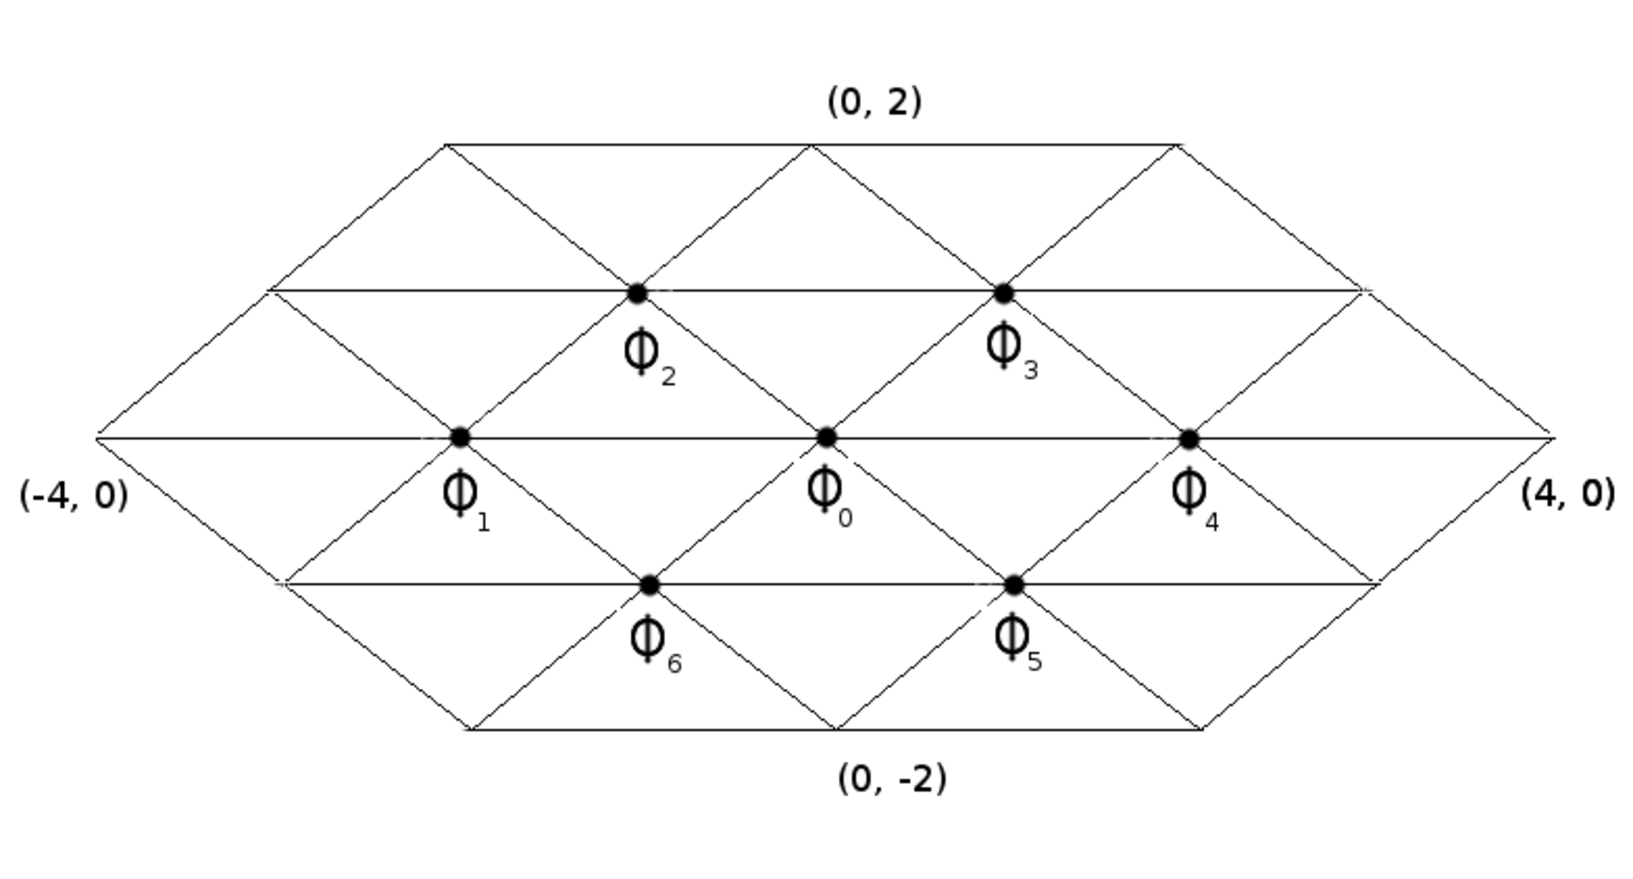
\includegraphics[scale=0.6]{finite_element_mesh}
    \end{center}
    \caption{Finite element mesh for the 7 hat functions centered at $(0, 0)$.}\label{mesh}
  \end{figure}

  As discussed in class, the weak formulation of the differential equation
  \label{laplace} is as follows
  \[
    \int_\Omega \triangledown u(x, y) \cdot \triangledown\phi_i(x, y) d\Omega = \int_\Omega (-x + 1)\phi_i(x, y)d\Omega \quad \text{for $i=0,\dots,6$}.
  \]
  We then require our approximation to satisfy this system, i.e.\
  \begin{align}\label{laplace_system}
    \sum_{j=0}^6 a_j \int_\Omega \phi_i(x, y) \phi_j(x, y) d\Omega = \int_\Omega (-x + 1)\phi_i(x, y)d\Omega \quad \text{for $i=0,\dots,6$}.
  \end{align}
  Equivalently, the system is given by $Ax = b$ where
  \[
    Ax =
    \renewcommand\arraystretch{1.5}
    \begin{bmatrix}
      \int_\Omega \phi_0(x,y)\phi_0(x,y) d\Omega & \int_\Omega \phi_0(x,y)\phi_1(x,y) d\Omega & \hdots & \int_\Omega \phi_0(x,y)\phi_6(x,y) d\Omega \\
      \int_\Omega \phi_1(x,y)\phi_0(x,y) d\Omega & \int_\Omega \phi_1(x,y)\phi_1(x,y) d\Omega & \hdots & \int_\Omega \phi_1(x,y)\phi_6(x,y) d\Omega \\
      \vdots & \vdots & \ddots & \vdots \\
      \int_\Omega \phi_6(x,y)\phi_0(x,y) d\Omega & \int_\Omega \phi_6(x,y)\phi_1(x,y) d\Omega & \hdots & \int_\Omega \phi_6(x,y)\phi_6(x,y) d\Omega \\

    \end{bmatrix}
    \begin{bmatrix}
      a_0 \\
      a_1 \\
      \vdots \\
      a_6
    \end{bmatrix}
  \]
  and
  \[
  b =
    \renewcommand\arraystretch{1.5}
  \begin{bmatrix}
    \int_\Omega (-x + 1) \phi_0(x,y) d\Omega \\
    \int_\Omega (-x + 1) \phi_1(x,y) d\Omega \\
    \vdots
    \int_\Omega (-x + 1) \phi_6(x,y) d\Omega
  \end{bmatrix}
  \]

  From our definitions of the basis functions, most of the entries in the matrix
  $A$ are 0. Specifically $a_{ij} = 0$ when there is no overlap in definition of
  the basis functions. Using $a_ij$ to denote $\int_\Omega \phi_i(x,y)\phi_j(x,y) d\Omega$,
  we see that
  \[
    A =
    \begin{bmatrix}
      a_{00} & a_{01} & a_{02} & a_{03} & a_{04} & a_{05} & a_{06} \\
      a_{10} & a_{11} & a_{12} & 0 & 0 & 0 & a_{16} \\
      a_{20} & a_{21} & a_{22} & a_{23} & 0 & 0 & 0  \\
      a_{30} & 0 & a_{32} & a_{33} & a_{34} & 0 & 0 \\
      a_{40} & 0 & 0  & a_{43} & a_{44} & a_{45} & 0 \\
      a_{50} & 0 & 0 & 0 & a_{54} & a_{55} & a_{56} \\
      a_{60} & a_{61} & 0 & 0 & 0 & a_{65} & a_{66} \\
    \end{bmatrix}.
  \]
  At the time of writing, the author regretfully informs that he was unable to fully solve this system,
  but the author does provide tools to calculate the equations of the plane for a given triangle
  in the following link:
  \url{https://github.com/gammadistribution/gradschool/tree/master/MATH635/final/programs/PDEs}

  Using these tools we can determine the equations of the plane for
  each triangle and calculate the integral over that triangle. Repeating this process
  for each domain of the basis functions we can determine the rest of the coefficients $a_{ij}$.
  The column vector is then computed similarly and we can use any desired technique
  to solve the system.
\end{proof}
